\chapter{Circuitos eléctricos}


\section{Teoremas de circuitos}


Una de las desventajas del análisis de circuitos mediante las eyes de Kirchhoff es que implica en gran medida circuitos complejos y tesiosos calculos. Se han desarrollado algunos teoremas para enfrentar esta compejidad. Entre estos teoremas están el teorema de Thevenin y el teorema de Norton como estos teoremas se aplican a circuitos lineales, primero se expondrá el concepto de lonealidad en los circuitos. También se expondrá el concepto de transformación de fuentes y máxima transferencia de potencia.

\subsection{Linealidad}



\subsection{Superposición}



\subsection{Transformación de fuentes}


\subsection{Teorema de Thevenin}

Teniendo en cuenta que la carga de un circuito en general es variable, el circuito entero debe vovler a analizarse. El teorema de thevenin evita este problema; proporciona una técnica mediante la cual la parte fija del circuito de reemplaza por un circuito equivalente. 

\begin{figure}[H]
    \centering
    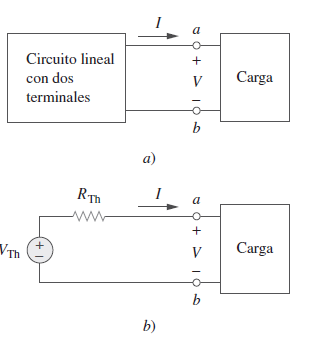
\includegraphics[scale=0.5]{Elect_circ/fig_circequiv.png}
\end{figure}

El teorema de Thevenin establece que un circuito lineal de dos terminales puede reemplazarse por un vurvuito equivalente que consta de una fuente de tension $V_{th}$ en seriie cin una resistentia $R_{th}$, donde $V_{th}$ es la tensión del circuito abierto en las terminales y $R_{th}$ es la entrada o la resistencia equivalente en las terminales cuando las fuentes están apagadas.

Para aplicar esta idea en el calculo de la resistencia de Thevenin se deben considerar dos casos

\begin{enumerate}
    \item Si la red no tiene fguentes dependientes, se apagan todas las fuentes independientes. $R_{th}$ es la resistencia equivalente de entrada que aparece entre las terminales.
    \item Si kla red tiene fuentes dependientes, se deben apagar todas las fuentes independientes, y se debe aplicar una tensión de prueba en las terminales. Se deberá medir la corriente resultante del circuito de prueba y la resistencia thevenin será $T_{th} = \frac{v_o}{i_o}$. De manera alternativa se puede aplicar una fuente de corriente de prueba y de manera análoga se determina la resistencia thévenin midiendo la tensión resultante en las terminales y dividiendo por la corriente de prueba.
\end{enumerate}

para el circuito equivalente de Thevenin 

\begin{figure}[H]
    \centering
    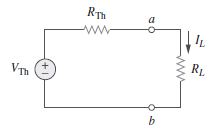
\includegraphics{Elect_circ/circ_f2.png}
\end{figure}

Se puede determinar la corriente $I_L$:

\begin{eqnarray*}
I_L = \frac{V_{Th}}{R_{Th}+R_L} \\
V_L = V_{Th} \frac{R_{L}}{R_{Th}+R_L}
\end{eqnarray*}

\subsection{Teorema de Norton}

El teorema de Norton establece que un circuito lineal de dos terminares puede reemplazarse por un curcuito equivalente que consta de una fuente de corriente $I_N$ en paralelo con un resistor $R_N$, sonde $I_n$ es la corriente de corto circuito a través de las terminales y $R_N$ es la resistencia de entrada o la resistencia equivalente en las terminales cuando las fuentes independientes están apagadas. \\

la resistencia de Norton y la resistencia de Thevenin son equivalentes. 

\begin{equation*}
R_n = R_{Tn}
\end{equation*}

Y por la transfornacion de fuentes:

\begin{equation*}
I_N = \frac{V{Th}}{R_{Th}}
\end{equation*}

\subsection{Máxima transferencia de potencia} \label{max_transf_pot}

\begin{figure}[H]
    \centering
    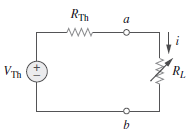
\includegraphics{Elect_circ/circ_f3.png}
\end{figure}

Para la figura anterior, podemos determinar la potencia que consume la carga $R_L$, esta potencia es

\begin{equation*}
p = i^2 R_L = \left( \frac{V_{Th}}{R_{Th}+R_L} \right)^2 R_L
\end{equation*}

Indica una función de $R_L$ que si se analiza se puede determinar que es nula en $R_L=0$ y $R_L \to \infty$, y tiene un máximo. Dicho máximo se puede determinar derivando la función e igualando a cero:

\begin{eqnarray*}
\frac{d p}{d R_L} = V_{Th}^{2} \left(  \frac{R_{Th}+R_L - 2R_L}{(R_{Th}+R_L)^3} \right) = 0 \\
R_l = R_{Th}
\end{eqnarray*}

Lo cual indica que para la máxima transferencia de potencia a la carga, esta debe tener una resistencia igual a la resistencia Thevenin del circuito. Si se cumple esto, esta potencia estará dada por

\begin{equation*}
p_{\text{max}} = \frac{V_{Th}^2}{4 R_{Th}}
\end{equation*}





\section{Potencia de ca}


La potencia es la cantidad más relevante en todos los sistemas de suministro de neregía. Cada máquina electrica tiene un valor de potencdia nominal que indica cuánta potencia requiere la misma. En principop se definene la potencia instantánea y la potencia promedio. después se presentarán otros conceptos de potendcia.


\subsection{Potencias instantánea y promedio} 
La potencia instantánea absorbida or un elemento de ircuito dse define como la multiplicación de la tensión y la corriente instantáneas.

\begin{equation*}
    p(t) = v(t) i(t)
\end{equation*}

Se puede concebir como la potencia absorbida por ele elemento un instante específico. Las cantidades instantánteas se suelen denotar con letras minúsculas. Su unidad de medida es el vatio (W). \\

Como ejemplo sea un circuito en cuyas dos terminales arbitrarias se mide la tensión y la corriente y estas son

\begin{eqnarray*}
    v(t) = V_m \cos (\omega t + \theta_v) \\
    I(t) = I_m \cos (\omega t + \theta_i)
\end{eqnarray*}

La potencia instantánea absorbida por el circuito es 

\begin{equation*}
p(t) = v(t) i(t) = V_m I_m \cos (\omega t + \theta_v) \cos (\omega t + \theta_i)
\end{equation*}

Aplicando la identidad trigonométrica 

\begin{equation*}
\cos A \cos B = \frac{1}{2} [\cos(A-B) + \cos (A+B)]
\end{equation*}

Se expresa la potencia instantánea de la siguiente forma

\begin{equation*}
p(t) = \frac{1}{2} V_m I_m \cos (\theta_v - \theta_i) + \frac{1}{2}V:m I_m \cos (2 \omega t + \theta_v + \theta_i)
\end{equation*}

Esto indica que la potencia instntanea tiene dos partes, una de las cuales es independiente ddel tiempo. Su valor depende de la diferencia de las fases de la tensión y de cirriente. La segunda parte es una fución sinussoidal cuya frecuencia es el doble de la frecuencia de la tensión y corriente.

La potencia instantánea es dif´´oicil de medir, por tanto aparece la potencia promedio. El watímetro que es el instrumento de medición de potencia, mide la potencia promedio. Esta potencia está dada por

\begin{equation*}
P = \frac{1}{T} \int_0^T p(t) dt
\end{equation*}

Aplicando la integral a la potencia sinusoidal de antes tenemos 

\begin{eqnarray*}
P = \frac{1}{2}V_m I_m \cos(\theta_v - \theta_i) \frac{1}{T} \int_0^T dt +  \frac{1}{2}V_m I_m \frac{1}{T} \int_0^T \cos (2 \omega t + \theta_v + \theta_i) dt 
\end{eqnarray*}

Esta expresión se simplifica a 

\begin{equation*}
P = \frac{1}{2} V_m I_m \cos (\theta_v - \theta_i)
\end{equation*}

Teniendo en cuenta la notación fasorial $\mathbf{V}=V_m \angle \theta_v$ e $\mathbf{I}=I_m\angle \theta_i$ podemos partir de que

\begin{eqnarray*}
\frac{1}{2} \mathbf{V} \mathbf{I}^{*} &=& \frac{1}{2}V_m I_m \angle (\theta_v - \theta_i) \\
 &=& \frac{1}{2}V_m I_m \left( \cos (\theta_v - \theta_i) + j \sin (\theta_v - \theta_i) \right)
\end{eqnarray*}

Por tanto podemos denotar de manera fasorial la potencia promedio así

\begin{equation*}
P = \frac{1}{2} \mathrm{Re}\{ \mathbf{VI^{*}} \} =  \frac{1}{2}V_m I_m \cos (\theta_v - \theta_i)
\end{equation*}

La potencia promedio disipada en una resistencia será

\begin{equation*}
P = \frac{1}{2} |\mathbf{I}|^2 R
\end{equation*}

Observe que cuando el desfase entre tensión y corriente es nulo, la potencia es máxima; indica un circuito puramente resistivo, si el desfase es máximo, es decir $90$ grados, la potencia promedio es nula y el circuito es puramente reactivo. 

\subsection{Máxima transferencia de potencia promedio}

En la sección \ref{max_transf_pot} se determinó cómo se maximiza la potencia entregada por una circuito a una carga mediante su equivalente de Thevenin. Se determino que la máxima transferencia se logra cuando la resistencia de  carga es igual a la resistencia de Thevenin.

Para los circuitos de corriente alterna, considere 

\begin{figure}[H]
    \centering
    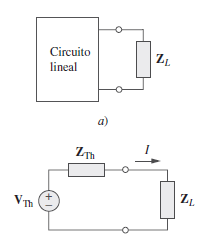
\includegraphics{Elect_circ/pot_f1.png}
\end{figure}

Las impedancias de thevenin y de carga pueden ser en forma triangular

\begin{eqnarray*}
\mathbf{Z}_{Th} = R_{Th} + j X_{Th} \\
\mathbf{Z}_{L} = R_{L} + j X_{L}
\end{eqnarray*}

La corriente que fluye por la carga será

\begin{equation*}
\mathbf{I} = \frac{\mathbf{V}_{Th}}{\mathbf{Z}_{Th} + \mathbf{Z}_L} = \frac{\mathbf{V}_{Th}}{ (R_{Th} + j X_{Th}) + (R_L + jX_L) }
\end{equation*}

Para este caso, la potencia promedio suministrada a la carga en este caso será

\begin{equation*}
P = \frac{1}{2}|\mathbf{I}|^2 R = \frac{|\mathbf{V}_{Th}|^2R_L/2}{(R_{Th} + R_L )^2 + (X_{Th} + X_L)^2}
\end{equation*}

El objetivo es ajustar los parámetros de carga $R_L$ y $X_L$ para que la potencia sea máxima. Para ello derivamos $P$ con respecto a $R_L$ y a $X_L$ e igualamos acero

\begin{eqnarray*}
\frac{\partial P }{\partial  X_L} = -\frac{|\mathbf{V}_{Th}|^2 R_L (X_{Th} + X_L)}{\left[ (R_{Th} + R_L)^2 + (X_{Th} + X_L)^2\right]^2} \\
\frac{\partial P }{\partial  R_L} = \frac{|\mathbf{V}_{Th}|^2 \left[(R_{Th} + R_L)^2 + (X_{Th} + X_L)^2 - 2R_L(R_{Th} + R_L)   \right]}{2 \left[ (R_{Th} + R_L)^2 + (X_{Th} + X_L)^2\right]^2}
\end{eqnarray*}


La solucion a este sistema de ecuaciones deja:

\begin{eqnarray*}
X_L = -X_{Th} \\
T_L = R_{Th}
\end{eqnarray*}

De manera que en conclusión, la impedancia de carga que maximiza la absorción de potencia de un circuito de CA es 

\begin{equation*}
\mathbf{Z}_L = \mathbf{Z}_{Th}^{*}
\end{equation*}

El complejo conjugado de la impedancia equivalente de Thevenin.

Esta potencia m+axima es 

\begin{equation*}
P_{\text{max}} = \frac{|\mathbf{V}_{Th}|^2}{8 T_{Th}}
\end{equation*}

En la situación en que la carga es puramente real, la condición para la máxima transferencia de potencia promedio deriva de 

\begin{equation*}
R_L = \sqrt{R_{Th}^2 + (X_{Th} + X_L)^2}
\end{equation*}

fijando $X_L=0$,

\begin{equation*}
R_L = \sqrt{R_{Th}^2 + (X_{Th})^2} = |\mathbf{Z}_{Th}|
\end{equation*}

\subsection{Valor efizar o RMS}

La idea del valor eficaz surge de la necesidad de medir la eficacia de una fuente de tensión o de corriente en el suministro de potencia a una carga resistiva.

El valor eficaz de una corriente periódica es la corriente de continua que suministraría la misma potencia promedio a una resistencia que la corriente periódica

\begin{figure}[H]
    \centering
    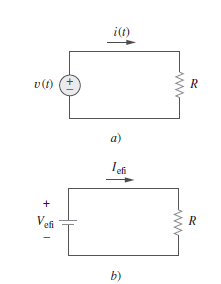
\includegraphics{Elect_circ/pot_f2.png}
\end{figure}

La potencia consumida por $R$ en el circuito AC es

\begin{equation*}
P=\frac{R}{T}\int_{0}^T i^2 dt
\end{equation*}

Mientras que la potencia en el circuito DC es

\begin{equation*}
P = I_{RMS}^2 R
\end{equation*}

Igualando estas dos potencial obtenemos que 

\begin{equation*}
I_{RMS} = \sqrt{\frac{1}{T}\int_0^T i^2 dt}
\end{equation*}

De la misma forma para la tensión eficaz, y para cualquier señal o función periódica en general. Aplicando este operador a una función sinusoidal se obtiene que el valor RMS es

\begin{equation*}
V_{RMS} = \frac{V_m}{\sqrt{2}} 
\end{equation*}

La potencia promedio se puede expresar en términos de tensión y corriente eficaces

\begin{eqnarray*}
p &=& \frac{1}{2}V_m I_m \cos (\theta_v - \theta_i) \\
&=& V_{RMS} I_{RMS} \cos (\theta_v - \theta_i) 
\end{eqnarray*}

Del mismo modo, la potencia promedio absorbida por una resistencia es

\begin{equation*}
P = \frac{V_{RMS}^2}{R}
\end{equation*}

\subsection{Potencia aparente y factor de potencia}

Como se vio anteriormente, podemos expresar la potencia promedio dadad dos señales de tensión y corriente de la siguiente forma

\begin{equation*}
P = V_{\textbf{RMS}} I_{\textbf{RMS}} \cos  (\theta_v - \theta_i) 
\end{equation*}

Sea $S=V_{\textbf{RMS}} I_{\textbf{RMS}}$, por tanto queda la anterior ecuación

\begin{equation*}
P = S  \cos  (\theta_v - \theta_i)
\end{equation*}

Se define $S$ como la \textbf{potencia aparente}, y el factor $ \cos  (\theta_v - \theta_i)$ es el \textbf{factor de potencia}.

La potencia aparente se llama así porque aparentemente la potencia debería ser el producto entre la tensión y la cdorriente, por analogia con los circuitos resistivos DC. Esta potencia se mide en volti-amperios (VA) para distinguirla de la potencia promedio o \textbf{real} medida en (W). \\

El ángulo $ (\theta_v - \theta_i)$ se conoce como el ángulo de factor de potencia. Si tomamos en cuenta el hecho de que en un elemento tenemos tensión $V_m \angle \theta_v$ y una corriente igual a $I_m \angle \theta_i$, la impedancia de dicho elemento es

\begin{equation*}
\mathbf{Z}=\frac{\mathbf{V}}{\mathbf{I}} = \frac{V_m \angle \theta_v}{I_m \angle \theta_i} = \frac{V_m}{I_m} \angle (\theta_v - \theta_i)
\end{equation*}

Por tanto el factor de potencia es el coseno del ángulo de la impedancia, alternativamente:

\begin{equation*}
\mathbf{Z}=\frac{V_\textbf{RMS}}{I_\textbf{RMS}} \angle (\theta_v - \theta_i)
\end{equation*}

El factor de potencia es el coseno del ángulo de desfase entre la tensión y la corriente, también es el coseno del ángulo de la impedancia de la carga. \\

Si el ángulo de desfase va desde -90 hasta 90, su coseno varía entre 0 y 1, cuando el factor de potencia es diferente de 1 se dice que está adelantado o atrasado. Un factor de potencia adelantado significa que la corriente se adelanta a la tensión, lo cual indica una carga caácitiva. Un factor de potencia atrasado significa que la corriente se atrasa de la tensión, lo cual implica una carga inductiva.

\begin{eqnarray*}
\mathbf{Z} = 25-j38.5 \Omega \text{denota un adelanto de fase, por tanto una carga capacitiva} \\
\mathbf{Z} = 25+j74 \Omega \text{denota un atraso de fase, por tanto una carga inductiva}
\end{eqnarray*}

Recordemos que 

\begin{eqnarray*}
\mathbf{Z} = R + j X_L \text{ o } R-jX_C \\
X_C = \frac{1}{\omega C} = \frac{1}{2 \pi f C}\\
X_L = \omega L = 2 \pi f L
\end{eqnarray*}

\subsection{Potencia compleja}

A lo largo de los años se han invertido considerables esfuerzos para expresar las relaciones de potencia en la forma más sencilla posible. Los ingenieros del área de potencia han acuñado el término potencia compleja, que emplean para hallar el efecto total de cargas en paralelo. La potencia compleja es importante en el análisis de potencia a causa de que contiene toda la información correspondiente a la potencia recibida por una carga dada. \\

Sea una carga $\mathbf{Z}$ cuya corriente es $\mathbf{I} = I_m \angle \theta_i$ y tensión $\mathbf{V}=V_m \angle \theta_v$. La potencia compleja $\mathbf{S}$ recibida por la carga AC es el producto de la tensión por el conjugado de la corriente

\begin{equation*}
\mathbf{S} = \frac{1}{2}\mathbf{V} \mathbf{I}^* = \mathbf{V}_{\text{RMS}} \mathbf{I}_{\text{RMS}}^{*} = \frac{V_\text{RMS}^2}{\mathbf{Z}^*}
\end{equation*}

donde 
\begin{eqnarray*}
\mathbf{V}_{\text{RMS}} = \frac{\mathbf{V}}{\sqrt{2}} \\
\mathbf{I}_{\text{RMS}} = \frac{\mathbf{I}}{\sqrt{2}}
\end{eqnarray*}

Veamos que la potencia compleja es

\begin{equation*}
\mathbf{S} = P + j Q
\end{equation*}

donde

\begin{eqnarray*}
P = \text{Re}\{ \mathbf{S} \} = I_\text{RMS}^2 R \\
Q = \text{Im} \{ \mathbf{S} \} = I_\textbf{RMS}^2 X
\end{eqnarray*}

Recordemos: \\

\textbf{P es la potencia promedio o real, Q es la potencia reactiva y $|\mathbf{S}|$ es la potencia aparente}

\begin{figure}[H]
    \centering
    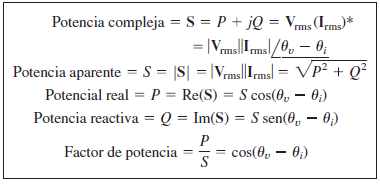
\includegraphics{Elect_circ/pot_f3.png}
\end{figure}

\subsection{Corrección del factor de potencia}

La mayoría de las cargas domésticas (como lavadoras, neveras, aire acondicionado, etc) y de las cargas industriales (como motores de inducción) son inductivasy operan con un factor de potencia bajo y atrasado. Aunque la naturaleza inductiva de la carga no puede modificarse, es posible incrementar su factor de potencia. \\

Dado que la mayoría de las cargas son inductivas, el factor de potencia de una carga se mejora o se corrige al instalar deliberadamente un capacitor en paralelo con la carga. El efecto de añadir el capacitor puede ilustrarse cin el truángulo de potencia o el diagrama fasorial de las corrientes implicadas.\\

La corrección del factor de potencia puede examinarse desde el siguiente punto de vista: considere un triángulo de potencia 

\begin{figure}[H]
    \centering
    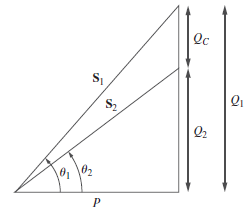
\includegraphics{Elect_circ/pot_f4.png}
\end{figure}

Si la carga inductiva original tiene la potencia aparente $S_1$ entonces

\begin{eqnarray*}
P = S_1 \cos \theta_1 \\
Q_1 = S_1 \sin \theta_1 = P \tan \theta_1
\end{eqnarray*}

Si se desea incrementar el factor de potencia de $\theta_1$ a $\theta_2$ sin alterar la potencia real ($P = S_2 \cos \theta_2$), la nueva potencia reactiva es 

\begin{equation*}
Q_2 = P \tan \theta_2
\end{equation*}

La reducción de la potencia reactiva es causada por el capacitor en derivación

\begin{equation*}
Q_c = Q_1 - Q_2 = P(\tan \theta_1 - \tan \theta_2)
\end{equation*}

pero como sabemos 

\begin{equation*}
Q_C = \frac{V_\text{RMS}^2}{X_C} = V_\text{RMS}^2 \omega C
\end{equation*}

\begin{equation*}
C = \frac{Q_C}{V_\text{RMS}^2 \ \omega} = \frac{P (\tan \theta_1 - \tan \theta_2)}{\omega V_\text{RMS}^2}
\end{equation*}

De manera análoga, para atrasar un factor de potencia adelantado, se debe conectar un inductor a la carga, y el valor de este inductor estará dado por

\begin{equation*}
L \frac{V_\text{RMS}^2}{\omega Q_L}
\end{equation*}


\section{Circuitos trifásicos}

Un circuito trifásico balanceado consta de tres fuentes de tensión con un desfase de 120 grados entre sí y que pueden estar conectados de las siguientes maneras

\begin{figure}
    \centering
    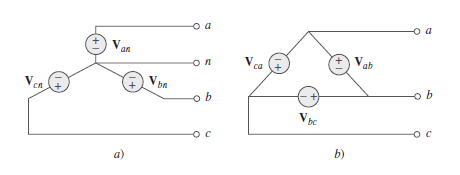
\includegraphics{Elect_circ/trif_f1.png}
\end{figure}

La primera configuración se llama estrella y tiene 4 terminales, una de las cuales se considera punto neutral. Las tensiones $\mathbf{V}_{an},\mathbf{V}_{bn},\mathbf{V}_{cn}$ se denominan tensiones de fase, y estas tensiones se dice que están balanceadas si tienen la misma frecuencia, amplitud y están desfasadas 120 gradeos entre sí. Esto implica que

\begin{equation*}
\mathbf{V}_{an} + \mathbf{V}_{bn} + \mathbf{V}_{cn} = 0
\end{equation*}

\begin{equation*}
|\mathbf{V}_{an}|=|\mathbf{V}_{bn}|=|\mathbf{V}_{cn}|
\end{equation*}

Existen dos formas en las que están configuradas las fases:

\begin{eqnarray*}
\mathbf{V}_{an} = V_P \angle 0^{o}  \\
\mathbf{V}_{bn} = V_P \angle -120^{o} \\
\mathbf{V}_{cn} = V_P \angle 120^{o}
\end{eqnarray*}

\begin{eqnarray*}
\mathbf{V}_{an} = V_P \angle 0^{o} \\
\mathbf{V}_{cn} = V_P \angle  -120^{o} \\
\mathbf{V}_{bn} = V_P \angle  120^{o}
\end{eqnarray*}

La primera se conoce como secuencia abc o positiva. La segunda secuencia se denomina acb o negativa.


Al igual que con el generador, las cargas también se pueden conectar en estrella o en fase. En una carga balanceada las tres impedancias tiene el mismo valor. En una carga balanceada en estrella

\begin{equation*}
\mathbf{Z}_1 = \mathbf{Z}_2 = \mathbf{Z}_3 = \mathbf{Z}_Y
\end{equation*}

en una carga balanceada en delta,

\begin{equation*}
\mathbf{Z}_a = \mathbf{Z}_b = \mathbf{Z}_c = \mathbf{Z}_{\Delta}
\end{equation*}

La relación entre ambos tipo de impedancia es

\begin{eqnarray*}
\mathbf{Z}_{\Delta} = 3 \mathbf{Z}_Y
\end{eqnarray*}

\subsection{Conexión estrella-estrella balanceada}

Considere una fuente trifásica en estrella conectada con una carga estrella balanceada, si se tiene en cuenta la impadancia interna o impedancia de fuente y la impedancia de línea, se puede considerar una impedancia de carga como la suma (serie) de impedancia de carga, línea y fuente.

Es evidente que se puede realizar la suma fasorial de las tensiones de fase para determinar los valores de tensiones de línea:

\begin{eqnarray*}
\mathbf{V}_{bc} = \mathbf{V}_{an} - \mathbf{V}_{bn} = \sqrt{3} V_p \angle 30^{o} \\
\mathbf{V}_{bc} = \mathbf{V}_{an} - \mathbf{V}_{bn} = \sqrt{3} V_p \angle 30^{o} \\
\mathbf{V}_{bc} = \mathbf{V}_{an} - \mathbf{V}_{bn} = \sqrt{3} V_p \angle 30^{o}
\end{eqnarray*}

La magnitud de las tensiones de línea es igual a $\sqrt{3}$ veces la magnitud de las tensiones de fase.

\subsection{Potencia en un sistema balanceado}

Considere ahora la potencia en un sistema trif+asico balanceado. Se comenzará examinando la potencia instantánea absorbida por la carga. Esto requiere que el análisis se realice en el dominio temporal. En na carga conectada en Y, las tensiones de fase son

\begin{eqnarray*}
v_{an} &=& \sqrt{2} V_P \cos \omega t \\
v_{bn} &=& \sqrt{2} V_P \cos (\omega t -120 ) \\
v_{cn} &=& \sqrt{2} V_P \cos (\omega t +120 )
\end{eqnarray*}

El factor $\sqrt{2}$ es necesario porque $V_P$ se definió como el valor RMS. $\mathbf{Z}_Y = Z \angle \theta$, las corrientes de fase se atrasan respecto a las tensiones de fase respectivas en $\theta$, es decir

\begin{eqnarray*}
i_a &=& \sqrt{2} I_P \cos (\omega t - \theta) \\
i_b &=& \sqrt{2} I_P \cos (\omega t - \theta - 120) \\
i_c &=& \sqrt{2} I_P \cos (\omega t - \theta + 120)
\end{eqnarray*}

La potencia instantánea total en la carga es la suma de las potencias instantáneas en las tres fases

\begin{equation*}
p = p_a + p_b + p_c = v_{AN}i_a + v_{BN} i_b + v_{CN} i_c
\end{equation*}

\begin{eqnarray*}
p &=& V_p I_p \left[ 3 \cos \theta + \cos (2 \omega t \theta) + \cos (2 \omega t - \theta - 240) + \cos(2 \omega t - \theta + 240) \right] \\
  & & \textbf{donde } \alpha = 2 \omega t - \theta \\
&=& V_pI_p \left[ 3 \cos \theta + \cos \alpha +2 \left( -\frac{1}{2} \right) \cos \alpha \right] \\
&=& 3V_pI_p \cos \theta
\end{eqnarray*}

note cómo la potencia instantánea es independiente del tiempo. Esto es verdad ya sea que la carga esté conectada en $Y$ o en $\Delta$. \\

La potencia promedio por fase es igual a $p/3$

\begin{equation*}
P_P = V_p I_p \cos \theta
\end{equation*}
 Y las potencias reactiva y aparente son 

\begin{eqnarray*}
Q_p = V_p I_p \sin \theta \\
S_p = V_p I_p
\end{eqnarray*}

  Finalmente la potencia compleja es

\begin{equation*}
\mathbf{S}_p = P_p + j Q_p = \mathbf{V}_p \mathbf{I}_p^{*}
\end{equation*}

La potencia total es la suma de las potencias promedio, así

\begin{equation*}
P = P_a + P_b + P_c = 3 P_p = 3 V_p I_p \cos \theta = \sqrt{3}V_L I_L \cos \theta
\end{equation*}

Tenga en cuenta que en estrella $I_P = I_L$, pero $V_L = \sqrt{3}V_P$ mientras que en $\Delta$ $V_L = V_P$ pero $I_L = \sqrt{3}I_P$. Así esta ecuación anterior se aplica en ambas configuraciones. Del mismo modo la potencia reactiva total es 

\begin{equation*}
Q = 3V_P I_P \sin \theta = 3 Q_P = \sqrt{3} V_L I_L \sin \theta 
\end{equation*}

 Y la potencia completa total es

\begin{eqnarray*}
\mathbf{S} &=& 3\mathbf{S}_p = 3 \mathbf{V}_P \mathbf{I}_P^{*} = 3I_P^2\mathbf{Z}_P = \frac{3 V_p^2}{\mathbf{Z}_P^{*}} \\
&=& P + j Q = \sqrt{3} V_L I_L \angle \theta
\end{eqnarray*}

Recordemos que estos valores son RMS y que el ángulo $\theta$ es el ángulo de la impedancia de la carga trifásica o de desfase entre tensión y corriente.
